%& C:\Users\CBalla\AppData\Roaming\TikzEdt\TikzEdt\023~1.0\TEMP_H~1
\begin{document}
\usetikzlibrary{arrows}
\begin{tikzpicture}[scale=0.7,transform shape]

 \node[anchor=south west,inner sep=0] at (0,0) {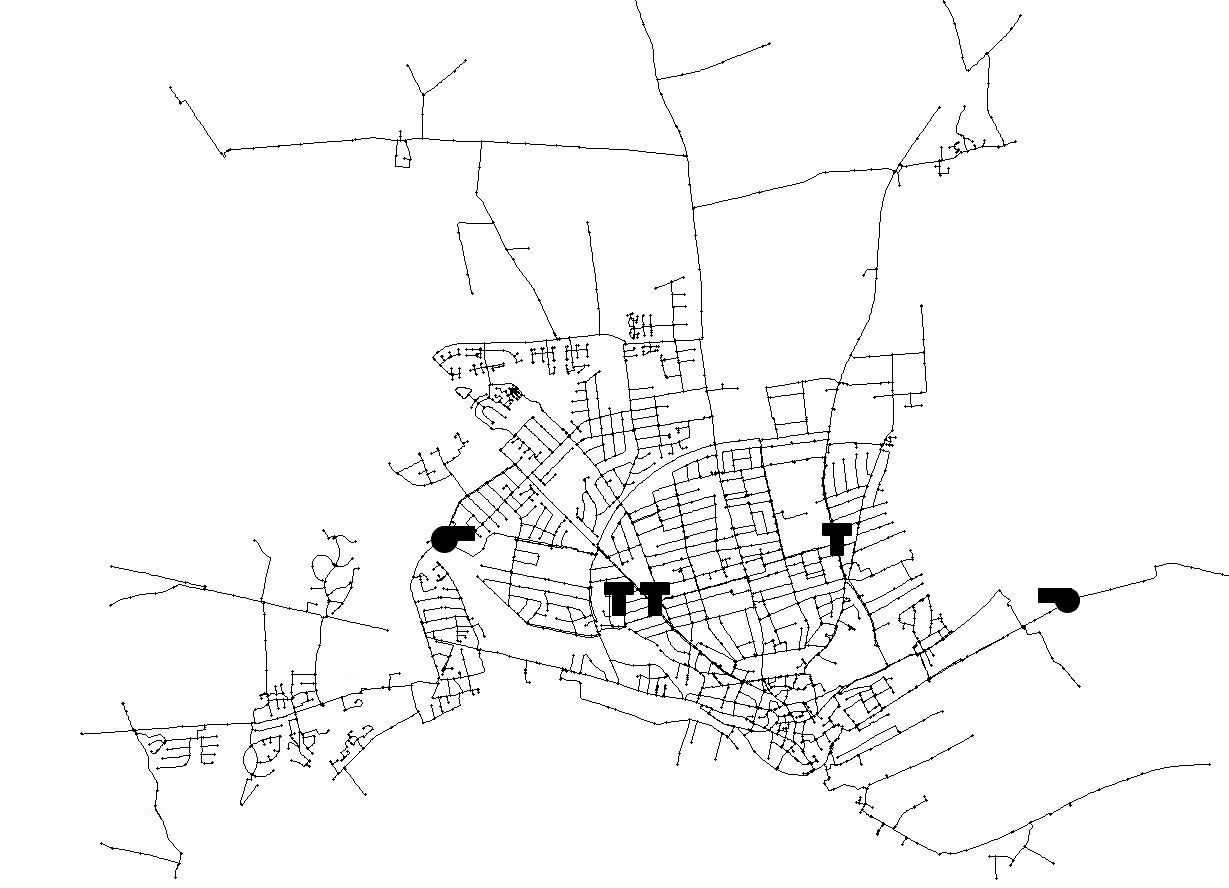
\includegraphics[width=\textwidth]{report/tikz/identification_map1}};
\node[black] at (11.4,4.75) {\footnotesize $\bm {\mathcal{W}_3}$};
\node[black] at (13.75,3.3) {\footnotesize $\bm {\mathcal{K}_2}$};
\node[black] at (4.7,4.65) {\footnotesize $\bm {\mathcal{K}_1}$};
\node[black] at (8.4,1) {\footnotesize $\bm {\mathcal{W}_2}$};
\node[black] at (6.8,1) {\footnotesize $\bm {\mathcal{W}_1}$};
\draw [-latex][thick](8.05,3.2) -- (8.4,1.35);
\draw [-latex][thick](7.55,3.2) -- (6.8,1.35);

\usetikzlibrary{calc}
\pgftransformreset
\node[inner sep=0pt,outer sep=0pt,minimum size=0pt,line width=0pt,text width=0pt,text height=0pt] at (current bounding box) {};
%add border to avoid cropping by pdflibnet
\foreach \border in {0.1}
  \useasboundingbox (current bounding box.south west)+(-\border,-\border) rectangle (current bounding box.north east)+(\border,\border);
\newwrite\metadatafile
\immediate\openout\metadatafile=\jobname_BB.txt
\path
  let
    \p1=(current bounding box.south west),
    \p2=(current bounding box.north east)
  in
  node[inner sep=0pt,outer sep=0pt,minimum size=0pt,line width=0pt,text width=0pt,text height=0pt,draw=white] at (current bounding box) {
\immediate\write\metadatafile{\p1,\p2}
};
\immediate\closeout\metadatafile
\end{tikzpicture}

\end{document}
